\documentclass[11pt,a4paper]{article}

\usepackage{main}
\usepackage{cours}

\renewcommand{\typedocument}{Cours}
\renewcommand{\classe}{5e}
\renewcommand{\titre}{Electricité}

\begin{document}

\pagination

\creertitre{Electricité}

\partie{Les dipôles}

Un \important{dipôle} est un composant électrique qui possède deux bornes. \\[10pt]
Certains dipôles sont des \important{générateurs} : ils fournissent de l’énergie électrique. \\[5pt]
\exemple{un générateur, une pile}. \\[10pt]
Certains dipôles sont des \important{récepteurs} : ils reçoivent et utilisent l’énergie électrique. \\[5pt]
\exemple{une lampe, un moteur}.

\partie{Circuit électrique et courant électrique}

Un \important{circuit électrique} est un ensemble de dipôles reliés par des fils électriques.

Il permet de transférer de l’énergie électrique d’un \important{générateur} vers un ou plusieurs \important{récepteurs}.

Pour fonctionner, un circuit doit former une \important{boucle fermée, afin que le courant circule}.

Le \important{courant a un sens} : il circule de la borne positive (+) vers la borne négative (–) du générateur.

\partie{Les matériaux conducteurs et isolants}

Certains matériaux laissent passer le courant : ce sont des \important{conducteurs} électriques.

\exemple{Tous les métaux (fer, aluminium, or, argent, cuivre, …) et le carbone.}

Certains matériaux ne laissent pas passer le courant : ce sont des \important{isolants} électriques.

\exemple{Plastique, bois, verre, papier}

\partie{Représenter un circuit : le schéma électrique}

Pour représenter un circuit simplement, on utilise un schéma électrique.

Dans un schéma électrique on doit :
\begin{itemize}
    \item représenter les dipôles par leur symbole et les fils électriques par des traits ;
    \item utiliser un crayon à papier et tracer les traits à la règle ;
    \item le dessiner en forme rectangulaire ;
    \item placer les dipôles sur les côtés du rectangle, jamais dans les coins.
\end{itemize}

\vspace{6pt}

\exemple{Schéma électrique d'un circuit avec une pile, une lampe et un interrupteur fermé.}

\begin{center}
    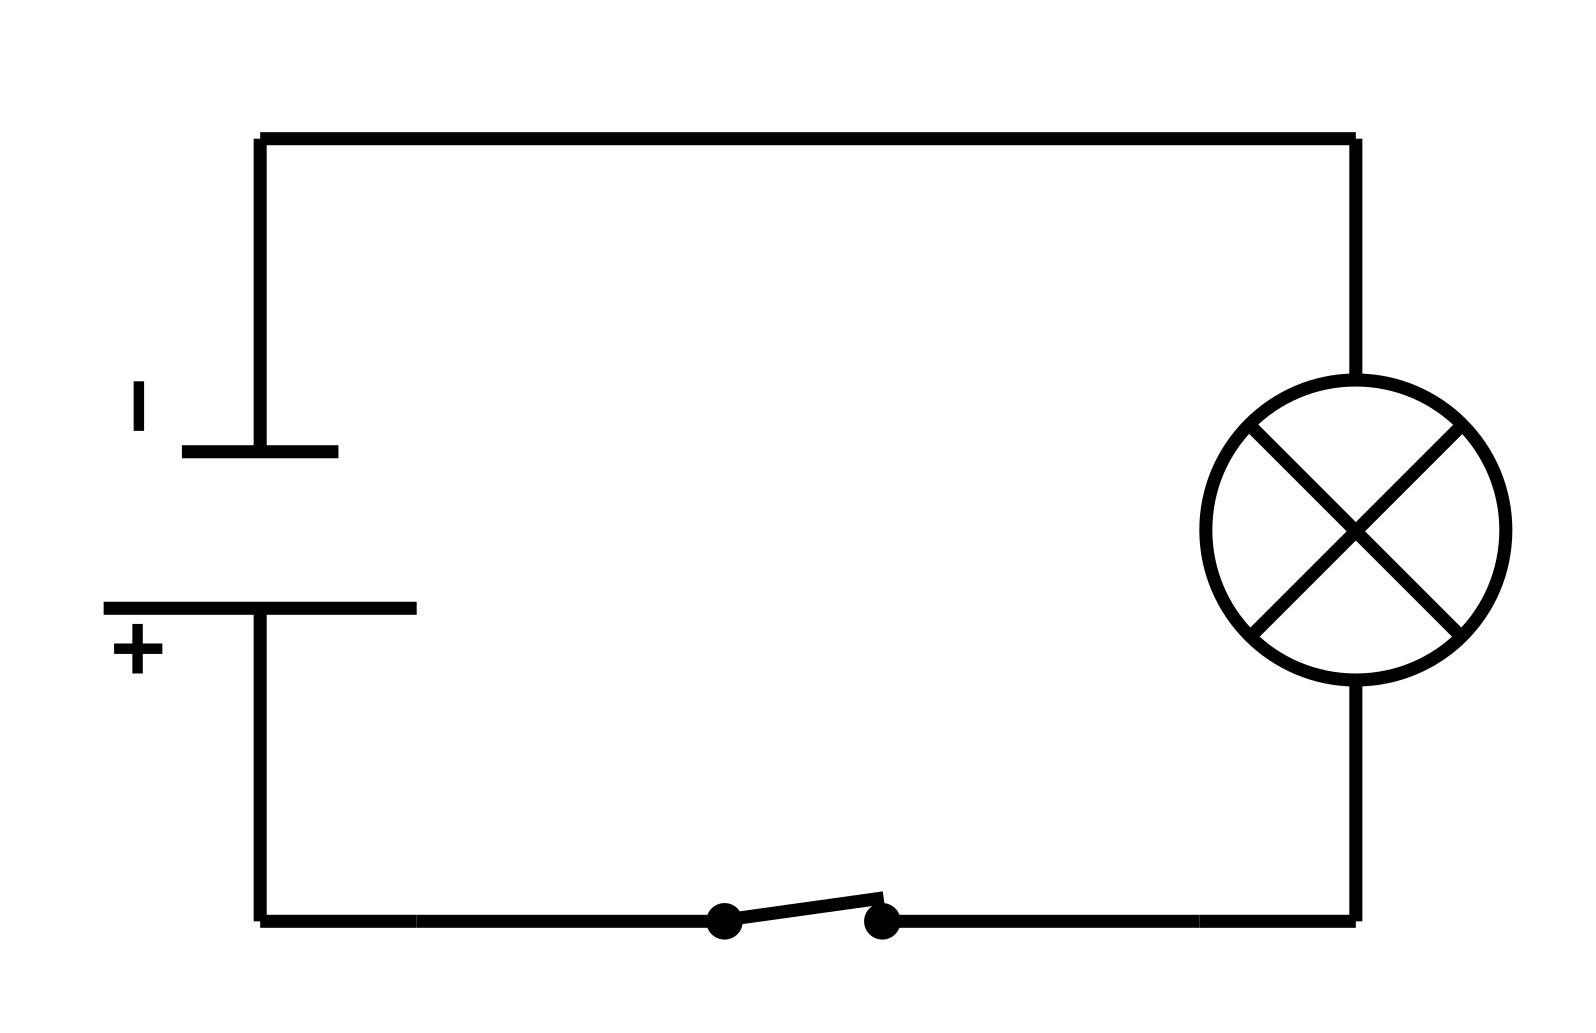
\includegraphics[width=6cm]{images/circuit.png}
\end{center}

\textbf{Voir le Document 5E4D - Dipôles électriques}

\newpage

\partie{Montages en série ou en dérivation}

\souspartie{Définitions}

\textbf{Montage en série :}
Montage constitué d’\important{une seule boucle}, où les dipôles sont placés les uns à la suite des autres.

\exemple{Schéma électrique d'un circuit en série}
\begin{center}
    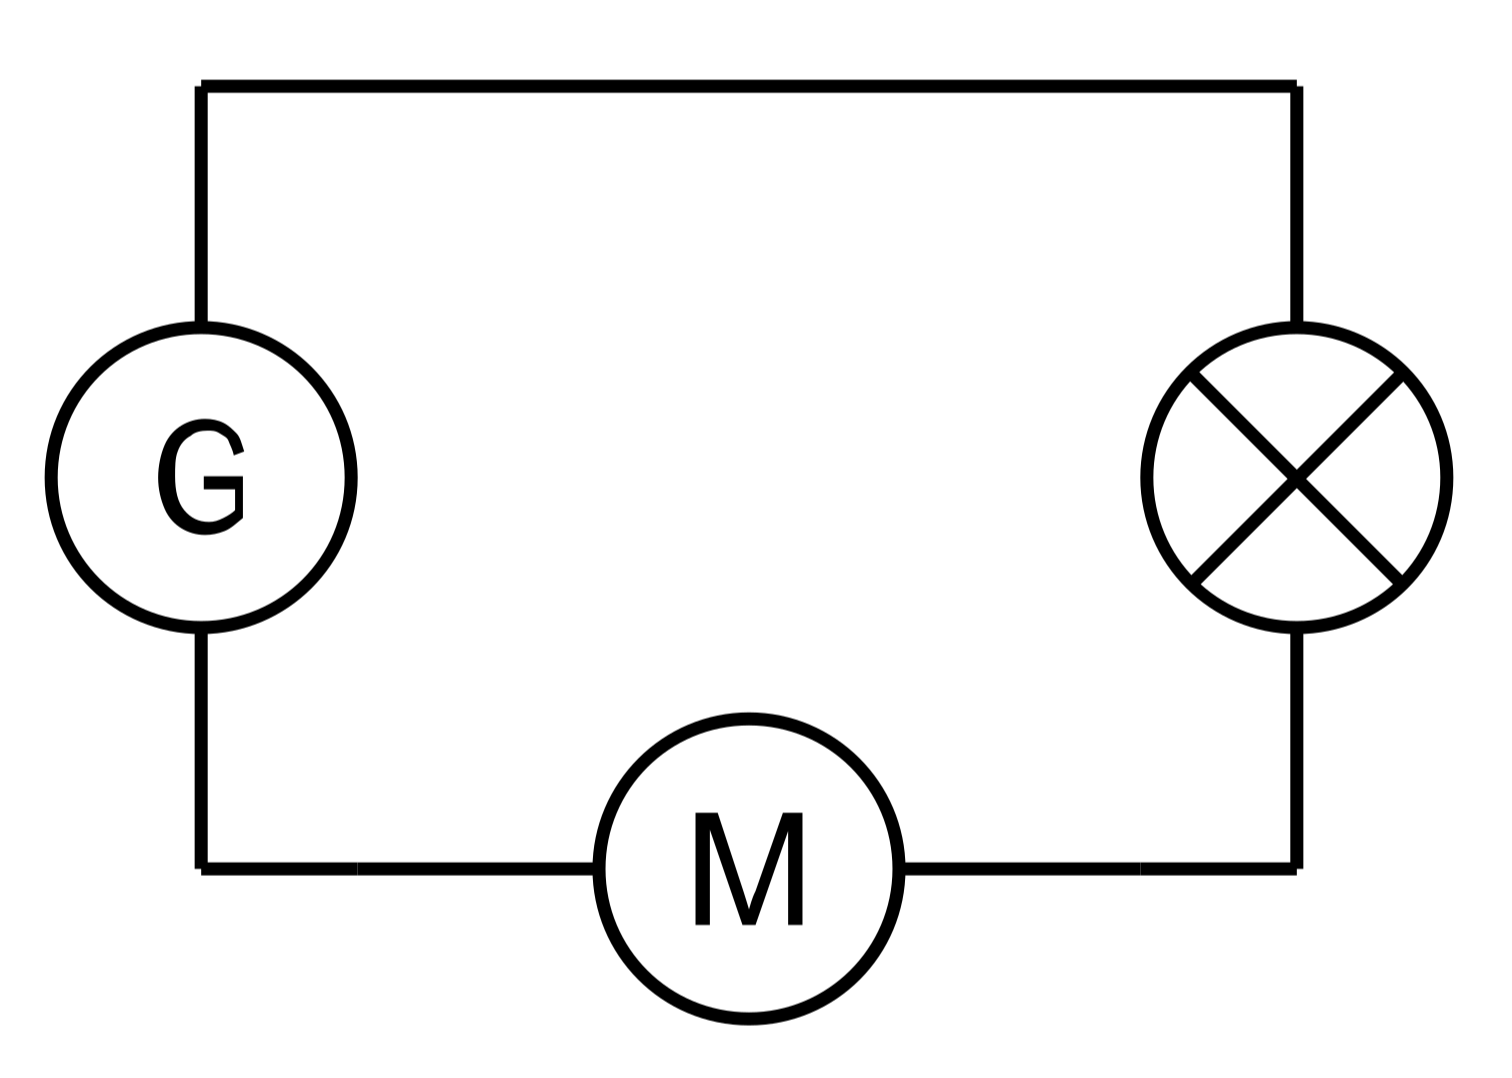
\includegraphics[width=6cm]{images/circuit serie.png}
\end{center}

\textbf{Montage en dérivation :}
Montage avec \important{plusieurs boucles}, où les dipôles sont branchés les uns aux bornes des autres

\exemple{Schéma électrique d'un circuit en dérivation}

\begin{center}
    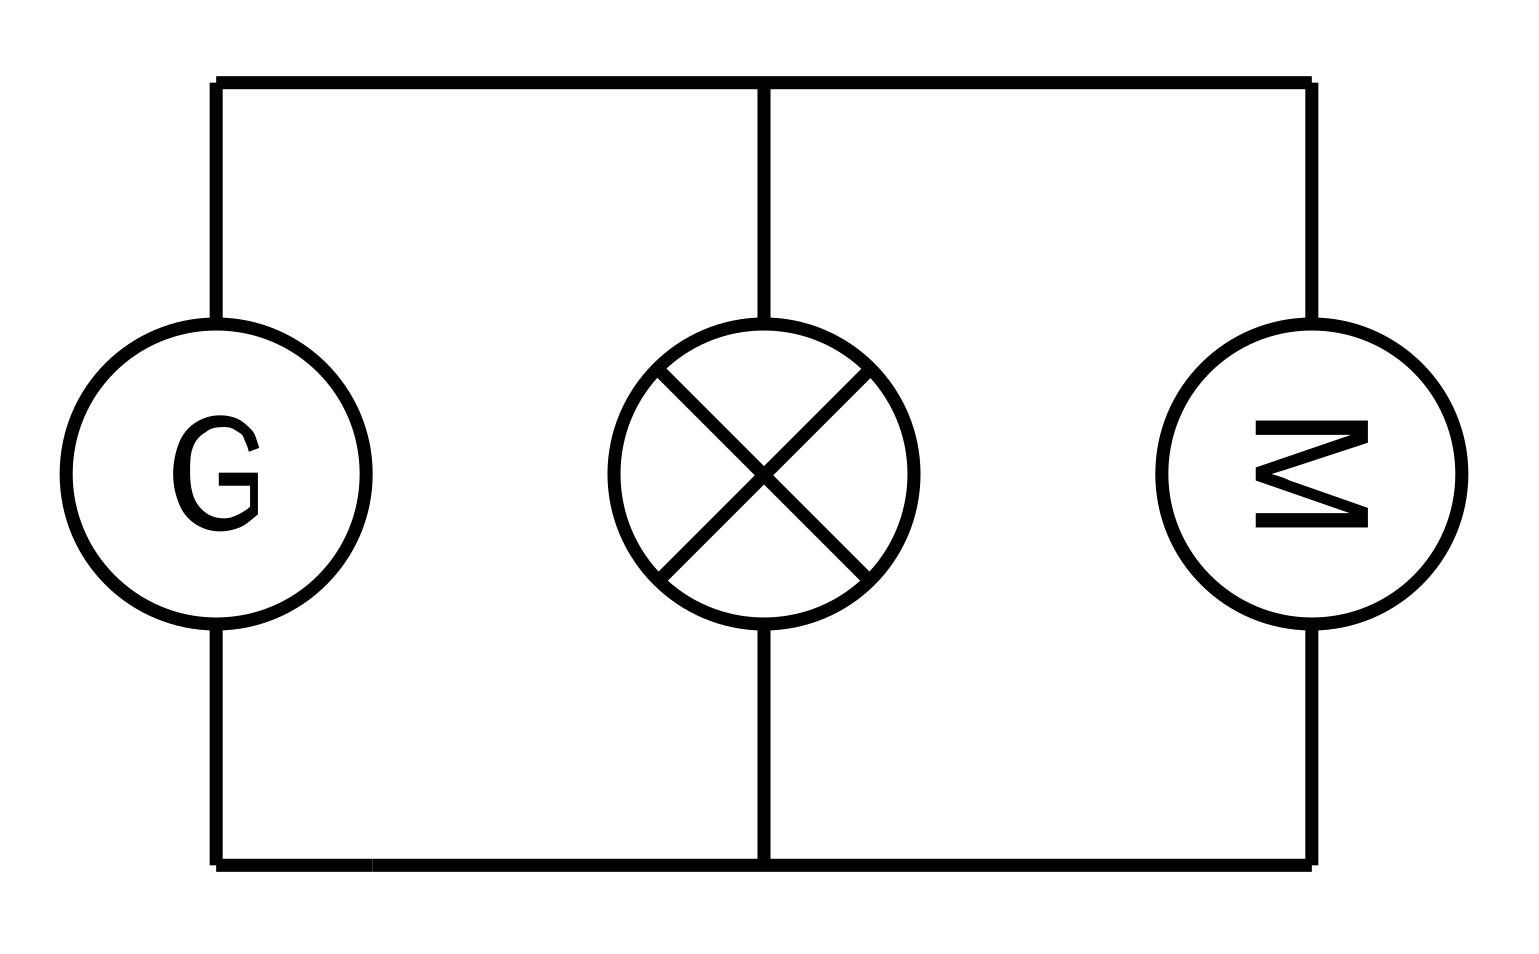
\includegraphics[width=6cm]{images/circuit derivation.png}
\end{center}

Les boucles correspondent aux rectangles du schéma électrique.

\souspartie{Expériences}

\textbf{Voir le Document 5E5D - Expériences}

\textbf{Conclusions : }

Dans un montage en série :
\begin{itemize}
    \item le nombre des dipôles a une importance sur le fonctionnement (expérience 1),
    \item si dipôle tombe en panne, les autres ne fonctionnent plus (expérience 2),
    \item l’ordre des dipôles n’a pas d’importance (expérience 3).
\end{itemize}

Dans un montage en dérivation, ni le nombre, ni l’ordre, ni l’état d’un dipôle n’a d’influence sur les autres dipôles (expériences 1/2/3). 

\souspartie{Court-circuit}

Le courant cherche toujours à passer par "le chemin" qui lui oppose le moins de résistance.

Lorsque les bornes d’un dipôle sont reliés par un fil, le courant passe par ce fil (il y a moins de résistance). On dit que le dipôle est en \important{court-circuit}. Le dipôle ne fonctionne plus (expérience 4).

\newpage

\partie{Les dangers du courant électrique et sécurité.}

\souspartie{Les dangers du court-circuit}

Le court-circuit d’un générateur ou d’une pile provoque une surchauffe qui \important{abîme l’appareil} et peut le détruire.

Dans une installation domestique, le court-circuit d’un appareil peut provoquer un \important{incendie}.

\souspartie{L’électrisation et l’électrocution}

Le corps humain n’est pas toujours un très bon conducteur d’électricité mais dans certains cas (lorsque notre peau est mouillée par exemple), un courant électrique peut le traverser.

Une personne est \important{électrisée} si elle est traversée par un courant électrique. Cela peut entraîner de graves brûlures, la tétanisation des muscles et des contractions rapides et irrégulières du cœur. Il y a \important{électrocution} lorsque le courant entraîne la mort.

La tension électrique est une grandeur que l’on peut mesurer dans un circuit électrique. Son unité est le volt (V). Plus elle est élevée, plus l’électrisation sera dangereuse.

\textbf{Voir le Document 5E7D - Electricité et sécurité}


\end{document}

